\documentclass[tikz,border=8pt]{standalone}
\usetikzlibrary{arrows.meta}

\begin{document}
\sffamily
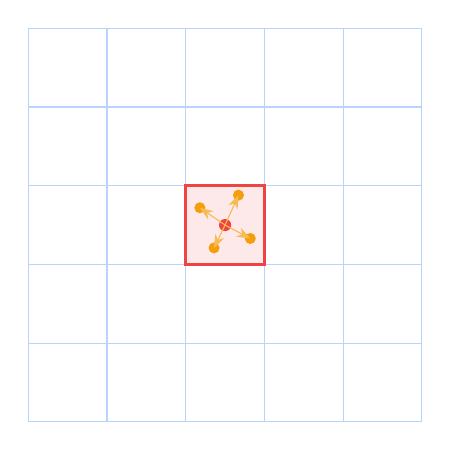
\begin{tikzpicture}[scale=1.0, >=Stealth]
  \definecolor{axisred}{RGB}{239,68,68}
  \definecolor{axisblue}{RGB}{59,130,246}
  \definecolor{rayorange}{RGB}{245,158,11}
  \definecolor{softgray}{RGB}{100,116,139}

  \draw[step=1, color=axisblue!35] (0,0) grid (5,5);
  \fill[axisred!12] (2,2) rectangle (3,3);
  \draw[axisred, line width=1.2pt] (2,2) rectangle (3,3);
  \fill[axisred] (2.5,2.5) circle (2.2pt);
  % \node[axisred, right] at (3.1,2.5) {center sample};

  \foreach \x/\y in {2.18/2.72,2.36/2.21,2.67/2.88,2.82/2.33} {
    \fill[rayorange] (\x,\y) circle (2pt);
    \draw[rayorange!70, ->] (2.5,2.5) -- (\x,\y);
  }

\end{tikzpicture}
\end{document}
